\documentclass[portrait,final,paperwidth=92cm, paperheight=152cm,  fontscale=0.277]{baposter}
%a0paper,
\usepackage{calc}
\usepackage{graphicx}
\usepackage{amsmath}
\usepackage{amssymb}
\usepackage{relsize}
\usepackage{multirow}
\usepackage{rotating}
\usepackage{bm}
\usepackage{url}
\usepackage{setspace}
\usepackage{graphicx}
\usepackage{multicol}
\usepackage{siunitx}
\usepackage{vwcol} 
\usepackage{varwidth}
\usepackage{tikz}
\usepackage{graphicx}
\usetikzlibrary{calc}
%\usepackage{times}
%\usepackage{helvet}
%\usepackage{bookman}
\usepackage{palatino}
\newcommand\Tstrut{\rule{0pt}{2.6ex}}         % = `top' strut

\newcommand{\captionfont}{\footnotesize}

\graphicspath{{images/}{../images/}}
\usepackage{tikz}
\usetikzlibrary{shapes.misc}
\usetikzlibrary{shapes,arrows,decorations.markings,shadows,positioning}
\usetikzlibrary{snakes,backgrounds,spy}
\usepackage{tcolorbox}
\newcommand{\SET}[1]  {\ensuremath{\mathcal{#1}}}
\newcommand{\MAT}[1]  {\ensuremath{\boldsymbol{#1}}}
\newcommand{\VEC}[1]  {\ensuremath{\boldsymbol{#1}}}
\newcommand{\Video}{\SET{V}}
\newcommand{\video}{\VEC{f}}
\newcommand{\track}{x}
\newcommand{\Track}{\SET T}
\newcommand{\LMs}{\SET L}
\newcommand{\lm}{l}
\newcommand{\PosE}{\SET P}
\newcommand{\posE}{\VEC p}
\newcommand{\negE}{\VEC n}
\newcommand{\NegE}{\SET N}
\newcommand{\Occluded}{\SET O}
\newcommand{\occluded}{o}
\renewcommand{\baselinestretch}{-1.5} 
%%%%%%%%%%%%%%%%%%%%%%%%%%%%%%%%%%%%%%%%%%%%%%%%%%%%%%%%%%%%%%%%%%%%%%%%%%%%%%%%
%%%% Some math symbols used in the text
%%%%%%%%%%%%%%%%%%%%%%%%%%%%%%%%%%%%%%%%%%%%%%%%%%%%%%%%%%%%%%%%%%%%%%%%%%%%%%%%

%%%%%%%%%%%%%%%%%%%%%%%%%%%%%%%%%%%%%%%%%%%%%%%%%%%%%%%%%%%%%%%%%%%%%%%%%%%%%%%%
% Multicol Settings
%%%%%%%%%%%%%%%%%%%%%%%%%%%%%%%%%%%%%%%%%%%%%%%%%%%%%%%%%%%%%%%%%%%%%%%%%%%%%%%%
\setlength{\columnsep}{1.5em}
\setlength{\columnseprule}{0mm}

%%%%%%%%%%%%%%%%%%%%%%%%%%%%%%%%%%%%%%%%%%%%%%%%%%%%%%%%%%%%%%%%%%%%%%%%%%%%%%%%
% Save space in lists. Use this after the opening of the list
%%%%%%%%%%%%%%%%%%%%%%%%%%%%%%%%%%%%%%%%%%%%%%%%%%%%%%%%%%%%%%%%%%%%%%%%%%%%%%%%
\newcommand{\compresslist}{%
	\setlength{\itemsep}{1pt}%
	\setlength{\parskip}{0pt}%
	\setlength{\parsep}{0pt}%
}

%%%%%%%%%%%%%%%%%%%%%%%%%%%%%%%%%%%%%%%%%%%%%%%%%%%%%%%%%%%%%%%%%%%%%%%%%%%%%%
%%% Begin of Document
%%%%%%%%%%%%%%%%%%%%%%%%%%%%%%%%%%%%%%%%%%%%%%%%%%%%%%%%%%%%%%%%%%%%%%%%%%%%%%
\begin{document}

%%%%%%%%%%%%%%%%%%%%%%%%%%%%%%%%%%%%%%%%%%%%%%%%%%%%%%%%%%%%%%%%%%%%%%%%%%%%%%
%%% Here starts the poster
%%%---------------------------------------------------------------------------
%%% Format it to your taste with the options
%%%%%%%%%%%%%%%%%%%%%%%%%%%%%%%%%%%%%%%%%%%%%%%%%%%%%%%%%%%%%%%%%%%%%%%%%%%%%%

\definecolor{silver}{cmyk}{0,0,0,0.3}
\definecolor{black}{cmyk}{0,0,0.0,1.0}
\definecolor{darkYellow}{cmyk}{0,0,1.0,0.5}
\definecolor{darkSilver}{cmyk}{0,0,0,0.1}

\definecolor{KTHBlue}{cmyk}{.71,.37,0.07,0}
\definecolor{KTHsilver}{cmyk}{0,0,0,0.35}
\definecolor{KTHbeige}{cmyk}{0,0.03,0.19,0.04}

\begin{poster}{
  % Poster Options
	% Show grid to help with alignment
	grid=false,
	columns=6,
	% Column spacing
	colspacing=1em,
	% Color style
	bgColorOne=white,
	bgColorTwo=white,
	borderColor=KTHBlue,
	headerColorOne=black,
	headerColorTwo=KTHBlue,
	headerFontColor=white,
	boxColorOne=white,
	boxColorTwo=KTHBlue,
	% Format of textbox
	textborder=roundedleft,
	% Format of text header
	eyecatcher=true,
	headerborder=closed,
	headerheight=0.15\textheight,
	%  textfont=\sc, An example of changing the text font
	headershape=roundedright,
	headershade=shadelr,
	headerfont=\Large\bf\textsc, %Sans Serif
	textfont={\setlength{\parindent}{0em}},
	boxshade=plain,
	%  background=shade-tb,
	background=plain,
	linewidth=2pt
}
% Eye Catcher
{
	
} 
% Title
{\bf\textsc{Bunch Length Measurements Using \\CTR 
		at the AWA with Comparison to Simulation}}%\vspace{0.1em}}
% Authors
{\vspace{1em}
	N. Neveu\textsuperscript{1}, L. Spentzouris, Illinois Institute of Technology, Chicago, IL, USA \\
	A. Halavanau, P. Piot\textsuperscript{2}, Northern Illinois University, DeKalb, IL, USA \\
	J. G. Power, E. Wisniewski, C. Whiteford, \textsuperscript{1} ANL, Lemont, IL, USA \\
	S. Antipov, Euclid Techlabs LLC, Solon, OH, USA \\
	\textsuperscript{2} also at Fermilab, Batavia, IL, USA \\
    }
% University logo
{% The makebox allows the title to flow into the logo, this is a hack because of the L shaped logo.
			%\makebox[3em][r]{
			\includegraphics[height=17em]{combo_logo_niu}%}

}


%%%%%%%%%%%%%%%%%%%%%%%%%%%%%%%%%%%%%%%%%%%%%%%%%%%%%%%%%%%%%%%%%%%%%%%%%%%%%%
\headerbox{AWA Facility}{name=problem,column=0,row=0, span=2, }{
%%%%%%%%%%%%%%%%%%%%%%%%%%%%%%%%%%%%%%%%%%%%%%%%%%%%%%%%%%%%%%%%%%%%%%%%%%%%%%
The photoinjector used for these studies consists of a gun and solenoids followed
by six accelerating cavities, see figure below. 
The 248 nm UV laser has a Full Width Half Maximum
(FWHM) duration ranging from 1.5 ps to 10 ps.
Typical operating charges are 1, 4, 10, and \SI{40}{nC}. 
While these are the most common operating modes, 
other charges have been requested 
and provided depending on the experiment.
Recent experiments include emittance exchange, 
structure tests, thermal emittance measurements, 
and two beam acceleration. 
The AWA laser system was upgraded with the microlens array (MLA) setup
that yields very transversely homogeneous bunches.
The effect of the MLA generated beam on the final electron 
bunch length is not yet investigated, therefore motivating
this work.
}

%%%%%%%%%%%%%%%%%%%%%%%%%%%%%%%%%%%%%%%%%%%%%%%%%%%%%%%%%%%%%%%%%%%%%%%%%%%%%%
\headerbox{Measurement Technique}{name=measure,column=2,row=0,span=4, bottomaligned=problem}{
%%%%%%%%%%%%%%%%%%%%%%%%%%%%%%%%%%%%%%%%%%%%%%%%%%%%%%%%%%%%%%%%%%%%%%%%%%%%%%
\begin{minipage}{0.48\textwidth}
	We performed autocorrelation scans of the CTR produced by an electron distribution.
	The CTR is transported into a Martin-Puplett interferometer (MPI)
	where it's split and directed into two MPI arms with a half-transparent pellicle.
	The CTR beams are then combined together at the exit of the MPI with the variable path difference.
	The resulting CTR intensity is registered with a liquid helium cooled IR Labs
	bolometer as a function of path difference.
	The path difference is then converted into time as $\Delta \tau = 2 \Delta x$.
	The resulting FWHM bunch duration is determined from the Gaussian fit of the interferogram.
	To alleviate charge fluctuations, we recorded 15 bolometer values for each data point.
	The data points outside of the 3$\sigma$ bracket were considered as outliers and discarded. 
\end{minipage}\hspace{0.25em}
\begin{minipage}{0.5\textwidth}
	\centering
	\vspace{-0.5em}
	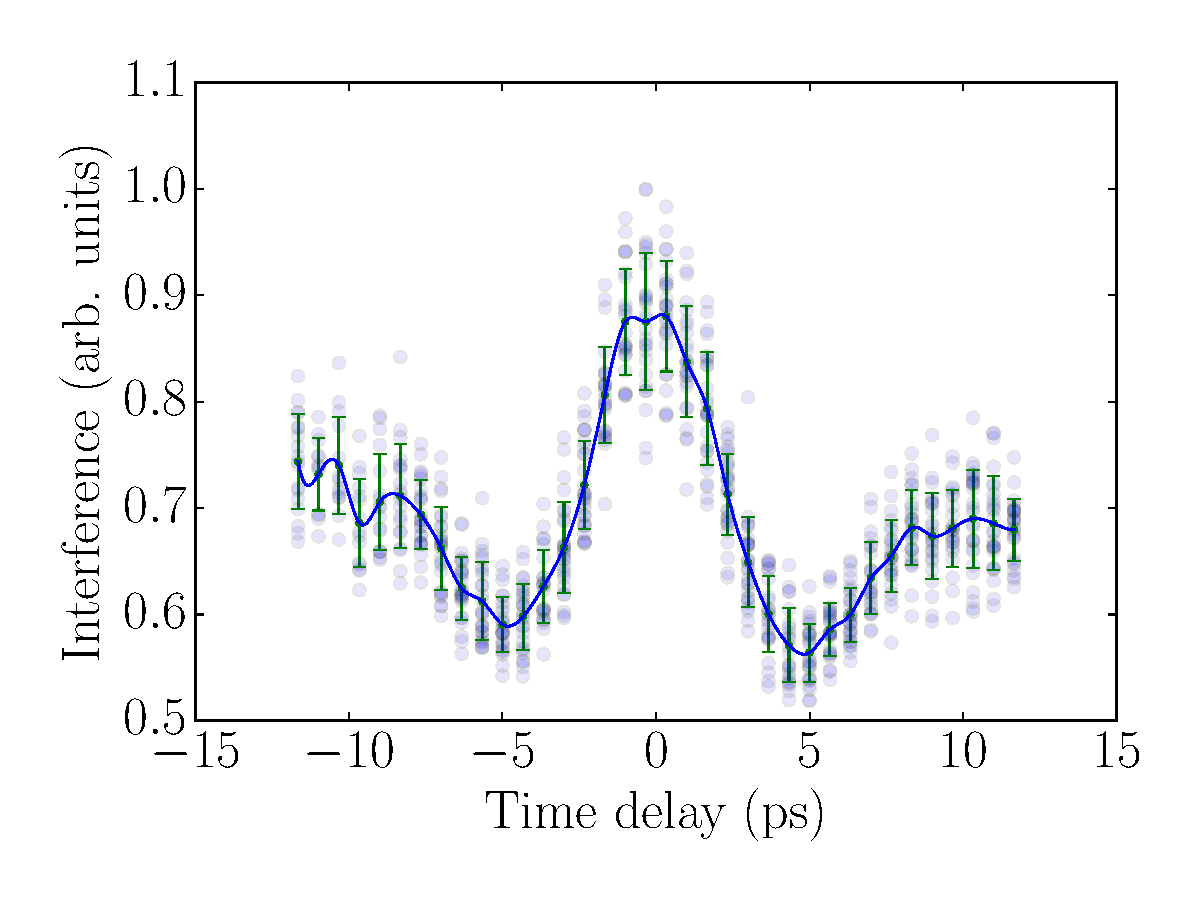
\includegraphics[width=1.0\linewidth]{images/THPMF048f1}
	An example interferogram for Q=30 nC and laser pulse FWHM of 1.5 ps.
\end{minipage}

}

%%%%%%%%%%%%%%%%%%%%%%%%%%%%%%%%%%%%%%%%%%%%%%%%%%%%%%%%%%%%%%%%%%%%%%%%%%%%%%
\headerbox{Beamline Layout}{name=beamline,column=0,below=problem, span=3}{%, bottomaligned=conclusion}{
%%%%%%%%%%%%%%%%%%%%%%%%%%%%%%%%%%%%%%%%%%%%%%%%%%%%%%%%%%%%%%%%%%%%%%%%%%%%%%
\noindent

\begin{center}
	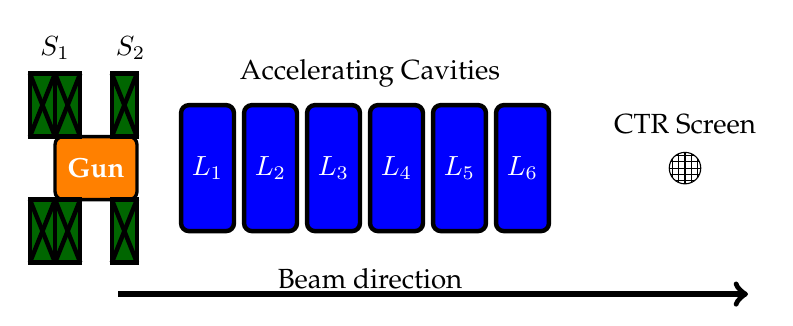
\begin{tikzpicture}[scale=0.8, text=black]
	\def \gunleft {-1.0}
\def \gunright {0.3}
\def \loneright {1.0}
\def \ltworight {2.0}
\def \lthreeright {3.0}
\def \lfourright {4.0}
\def \lfiveright {5.0}
\def \lsixright {6.0}
\def \quadone {7.5}

%Line between kicker and septum
\node[] at (4.0,-0.75) {Beam direction};
\draw[line width=0.75mm, ->] (0.0,-1.0) -- (10,-1.0);

\draw[fill=orange, very thick, rounded corners =0.1cm] (\gunleft,0.5)rectangle (\gunright,1.5) node[pos=.5, white] {\textbf{Gun}} ;
%S1
\node[] at (-1,2.9) {$S_1$};
\draw[ultra thick, fill=black!60!green] (-1.4,-0.5)rectangle  (-1.0,0.5) node[pos=.5, white] {} ;
\draw[black, ultra thick] (-1.4,-0.5) -- (-1.0,0.5);
\draw[black, ultra thick] (-1.4,0.5) -- (-1.0,-0.5);
\draw[ultra thick, fill=black!60!green] (-1.4,1.5)rectangle  (-1.0,2.5) node[pos=.5, white] {} ;
\draw[black, ultra thick] (-1.4,1.5) -- (-1.0,2.5);
\draw[black, ultra thick] (-1.4,2.5) -- (-1.0,1.5);
%S2
\draw[ultra thick, fill=black!60!green] (-1.0,-0.5)rectangle  (-0.6,0.5) node[pos=.5, white] {} ;
\draw[black, ultra thick] (-1.0,-0.5) -- (-0.6,0.5);
\draw[black, ultra thick] (-1.0,0.5) -- (-0.6,-0.5);
\draw[ultra thick, fill=black!60!green] (-1.0,1.5)rectangle  (-0.6,2.5) node[pos=.5, white] {} ;
\draw[black, ultra thick] (-1.0,1.5) -- (-0.6,2.5);
\draw[black, ultra thick] (-1.0,2.5) -- (-0.6,1.5);

%S3
\node[] at (0.2,2.9) {$S_2$};
\draw[ultra thick, fill=black!60!green] (-0.1,-0.5) rectangle  (0.3,0.5) node[pos=.5, white] {};
\draw[black, ultra thick] (-0.1,-0.5) -- (0.3,0.5);
\draw[black, ultra thick] (-0.1,0.5) -- (0.3,-0.5);
\draw[ultra thick, fill=black!60!green] (-0.1,1.5) rectangle  (0.3,2.5) node[pos=.5, white] {};
\draw[black, ultra thick] (-0.1,1.5) -- (0.3,2.5);
\draw[black, ultra thick] (-0.1,2.5) -- (0.3,1.5);
%Linac drawings 
\node[] at (4,2.5) {Accelerating Cavities};
\draw[fill=blue, ultra thick, rounded corners =0.1cm] (\loneright,0)rectangle  ({\loneright+0.84},2) node[pos=.5, white] {$L_1$} ;
\draw[fill=blue, ultra thick, rounded corners =0.1cm] (\ltworight,0)rectangle  ({\ltworight+0.84},2) node[pos=.5, white] {$L_2$};
\draw[fill=blue, ultra thick, rounded corners =0.1cm] (\lthreeright,0)rectangle ({\lthreeright+0.84},2) node[pos=.5, white] {$L_3$};
\draw[fill=blue, ultra thick, rounded corners =0.1cm] (\lfourright,0)rectangle ({\lfourright+0.84},2) node[pos=.5, white] {$L_4$};
\draw[fill=blue, ultra thick, rounded corners =0.1cm] (\lfiveright,0)rectangle ({\lfiveright+0.84},2) node[pos=.5, white] {$L_5$};
\draw[fill=blue, ultra thick, rounded corners =0.1cm] (\lsixright,0)rectangle ({\lsixright+0.84},2) node[pos=.5, white] {$L_6$};

%current optimization point
%\node[draw, fill=yellow, star, star points=5, star point ratio=0.6, minimum size=0.1cm]
%at (12.5,1.0) {$z_1$};
\node[] at (9,1.7) {CTR Screen};
\clip[draw] (9,1) circle (0.25cm);
\draw[step=1mm] (-1,-1) grid (10,10);

%Line between kicker and septum
\draw[very thick] (13.25,0.2) -- (14.5,-0.5);


%Line between septum and dipole
\draw[very thick] (15.6,-0.5) -- (16.5,-0.5);




	\end{tikzpicture}	
	
	\vspace{1em}
	Beam line layout at the AWA.
\end{center}

%\includegraphics[width=0.7\textwidth]{NN_range1.png}\includegraphics[width=.3\textwidth]{NN_train.png}\\
}

%%%%%%%%%%%%%%%%%%%%%%%%%%%%%%%%%%%%%%%%%%%%%%%%%%%%%%%%%%%%%%%%%%%%%%%%%%%%%%
\headerbox{Simulations}{name=sims,below=sims, below=measure, column=3,row=0,span=3}{
%%%%%%%%%%%%%%%%%%%%%%%%%%%%%%%%%%%%%%%%%%%%%%%%%%%%%%%%%%%%%%%%%%%%%%%%%%%%%%
\noindent
Simulations of the AWA beam line 
were performed with the code and OPAL.
Input parameters for the simulations are shown in the table below.
Note that on crest refers to the phase of max energy gain.
In the case of the gun, a -~$5^{\circ}$ phase is measured 
w.r.t the peak rf voltage.

\begin{center}
	Simulation Parameters
	\vspace{3.5em}
	\begin{singlespace}
		\begin{tabular}{lcc}
			\hline%\toprule
			\textbf{Parameter} & \textbf{Low Charge}  & \textbf{High Charge} \\
			\hline%\midrule
			Charge       & 0.3, 0.7, \SI{1.3}{nC}        & \SI{30}{nC}    \\ %[3pt]
			Gun Gradient & \SI{65}{MV/m}     & \SI{65}{MV/m}  \\ %[3pt]
			Gun Phase    & \SI{0}{}$^{\circ}$ & \SI{-5}{}$^{\circ}$ \\		 
			$S_1$        & \SI{230}{A}		 & \SI{500}{A}	  \\
			$S_2$		 & \SI{150}{A}   	 & \SI{235}{A}		 \\
			Linac Phases & On crest          & On crest       \\
			Laser FWHM   & \SI{1.5}{ps}      & \SI{1.5}{ps}   \\ %[3pt]
			Laser Radius & \SI{2}{mm}        & \SI{9}{mm}     \\
			\hline%\bottomrule
		\end{tabular}
	\end{singlespace}
\end{center}

Four scenarios were simulated, three low charge cases at 0.3, 0.7, and \SI{1}{nC}, and a 
high charge case at \SI{30}{nC}. 
These charges and input parameters were specifically chosen to 
match experimental measurements that had taken place or would 
take place in the future. Each simulation was run with 10,000 particles 
on 8 cores, and ran 2.5 minutes to reach a z location of \SI{17}{m}.
Prior work indicates the bunch length is not 
very sensitive to the number of particles or grid size. 
We expected charge, energy,
and laser parameters to have the most impact on the simulation values.
}

%%%%%%%%%%%%%%%%%%%%%%%%%%%%%%%%%%%%%%%%%%%%%%%%%%%%%%%%%%%%%%%%%%%%%%%%%%%%%%
\headerbox{Results}{name=results,column=3,below=sims, span=3}{%, bottomaligned=conclusion}{
%%%%%%%%%%%%%%%%%%%%%%%%%%%%%%%%%%%%%%%%%%%%%%%%%%%%%%%%%%%%%%%%%%%%%%%%%%%%%%
\noindent
While, we do not have an exact match, the results follow the same trends.
The discrepancies indicate there are still adjustments that can be made
to the simulation model. We will continue to try to improve agreement
as more of these measurements are made.
Note, the table gives bunch duration, and the plot gives bunch length for the same data.
	
	\begin{center}
		Experimental Measurements
		\vspace{3em}
		\begin{singlespace}
			\begin{tabular}{rcc}
				\hline%\toprule
				\textbf{Charge} & \textbf{Bunch Dur. (RMS)} & \textbf{Laser spot size}  \\
				\hline%\midrule
				\SI{0.3}{nC} & \SI{2.2}{ps} & 4 mm    \\ %[3pt]
				\SI{0.7}{nC} & \SI{2.6}{ps} & 4 mm   \\ %[3pt]
				\SI{1.3}{nC} & \SI{2.6}{ps} & 4 mm    \\
				\SI{30}{nC}  & \SI{4.1}{ps} & 9 mm \\ %[3pt]
				\hline%\bottomrule
			\end{tabular}
		\end{singlespace}
	\end{center}
	


\begin{center}
	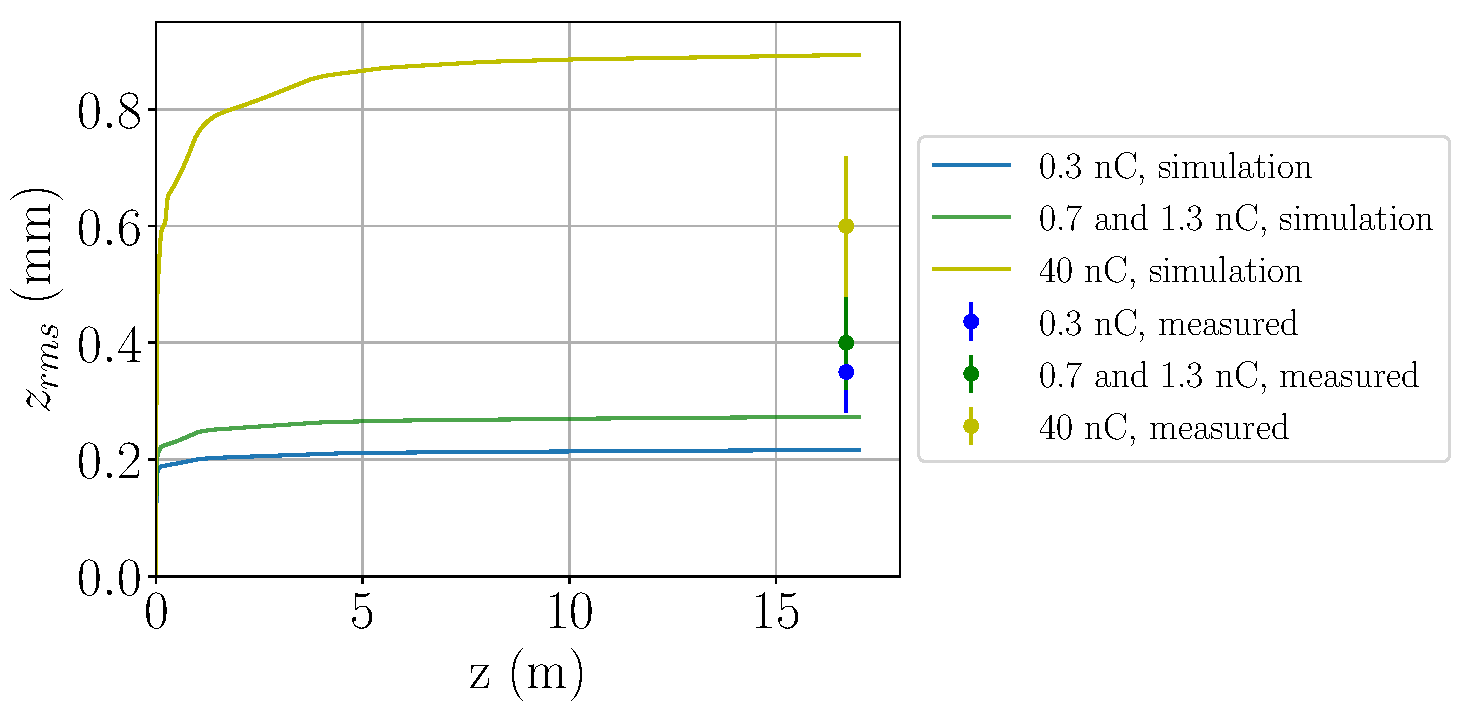
\includegraphics[width=1\linewidth]{images/THPMF048f5}
	
Comparison of simulations and experimental measurements.
\end{center}

}

%%%%%%%%%%%%%%%%%%%%%%%%%%%%%%%%%%%%%%%%%%%%%%%%%%%%%%%%%%%%%%%%%%%%%%%%%%%%%%
\headerbox{Experimental Setup}{name=exp,column=0,below=beamline, span=3}{%, bottomaligned=conclusion}{
%%%%%%%%%%%%%%%%%%%%%%%%%%%%%%%%%%%%%%%%%%%%%%%%%%%%%%%%%%%%%%%%%%%%%%%%%%%%%%
\noindent
\vspace{-1em}
\begin{center}
\begin{tikzpicture}[every node/.style={anchor=south west,inner sep=0pt},x=1mm, y=1mm,]   
\node (fig1) at (0,0)
{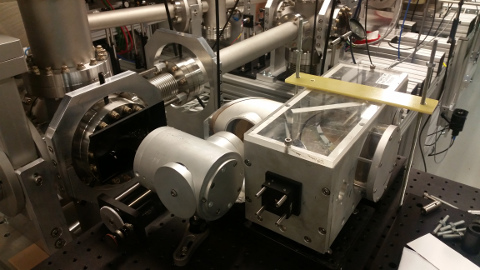
\includegraphics[width=0.8\textwidth]{images/THPMF048f3}};
\node[fill=white, inner sep=2pt] (txt2) at (35,15) {Interferometer};
\node[fill=white, inner sep=2pt, rotate=26] (txt2) at (18,19.5) {Slit};	
\node[fill=white, inner sep=2pt, rotate=20] (txt2) at (13,27) {Window};

\node (fig2) at (0,-55)
{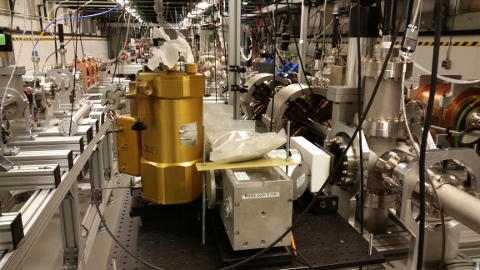
\includegraphics[width=0.8\textwidth]{images/THPMF048f4}};
\node[fill=white, inner sep=2pt] (txt2) at (35,-42) {Interferometer};	
\node[fill=white, inner sep=2pt] (txt2) at (55,-25) {Window};	
\node[fill=white, inner sep=2pt] (txt2) at (22,-15) {Bolometer};
\end{tikzpicture}
 
\end{center}


IR labs bolometer and MPI interferometer used in the experiment
to capture CTR light as it exited a window on the beam line.
\vspace{1em}

Bunches were allowed to propagate freely to the 
CTR screen. The only focusing elements used were solenoids $S_1$ and
$S_2$. As the bunches passed the CTR screen, light was
emitted through a window located next to the screen. 
A slit was used to prevent
background x-rays from reaching the bolometer.
After passing the slit, the CTR propagated to the 
interferometer. 
A remotely movable stage inside the interferometer was swept, 
and the resulting combined signal fed to the bolometer. 
Periodic refilling of the helium was required throughout the day in order
to keep the bolometer at \SI{4}{K}. 
}

%%%%%%%%%%%%%%%%%%%%%%%%%%%%%%%%%%%%%%%%%%%%%%%%%%%%%%%%%%%%%%%%%%%%%%%%%%%%%%
\headerbox{Conclusion}{name=con,column=3,above=bottom, below=results, aligned=ref, span=3}{%
%%%%%%%%%%%%%%%%%%%%%%%%%%%%%%%%%%%%%%%%%%%%%%%%%%%%%%%%%%%%%%%%%%%%%%%%%%%%%%
We performed experimental measurements of the electron bunch 
length using CTR and scanning interferometer technique.
The data was analyzed and compared to OPAL simulations.
The bunch length for the cases of 1 and \SI{30}{nC} is reported.
We note a decent agreement between the simulations and 
experimental results. The experimental setup will be used in the future
AWA CTR studies. 
}
%%%%%%%%%%%%%%%%%%%%%%%%%%%%%%%%%%%%%%%%%%%%%%%%%%%%%%%%%%%%%%%%%%%%%%%%%%%%%%
\headerbox{Acknowlegements}{name=ref,column=0,above=bottom, below=exp, span=3}{%
%%%%%%%%%%%%%%%%%%%%%%%%%%%%%%%%%%%%%%%%%%%%%%%%%%%%%%%%%%%%%%%%%%%%%%%%%%%%%%
\noindent 
We gratefully acknowledge the computing resources
provided on Bebop, a HPC cluster operated by the LCRC at ANL.
This work is supported by the U.S. DOE, OS,  
contract DE-AC02-06CH11357 and grant DE-SC0015479. 
Travel to IPAC'18 supported by the United States National Science Foundation, 
the Division of Physics of Beams of the American Physical Society, and TRIUMF.
\vspace{-1em}
\hfill
\begin{center}
	\includegraphics[width=0.125\textwidth]{logos/nsf}\hspace{1em}
	\includegraphics[width=0.4\textwidth]{logos/DOE_logo_color_cmyk}\hspace{1em}
	\includegraphics[width=0.125\textwidth]{logos/aps-logo}
\end{center}
}




\end{poster}%
%
\end{document}
